% !TeX program = xelatex
\documentclass{beamer}
\usepackage[UTF8]{ctex}
\usepackage{graphicx}
\usepackage{booktabs}
\usepackage{multirow}
\usepackage{hyperref}
\usepackage{amsmath,amssymb}
\usepackage{tikz}
\usetikzlibrary{shapes,arrows,positioning}

% 复用你第一阶段的主题配置(相对路径)
\input{../../新芽计划更改版/config.tex}
\useSmallCircleItem

% 基本信息
\title{新芽计划第二阶段汇报:Jittor 框架复现与对齐}
\author{柯云超}
\institute{南开大学}
\date{\\GitHub: https://github.com/kyc001}

\begin{document}
% 封面
\begin{frame}
  \titlepage
\end{frame}

% 目录
\begin{frame}{目录}
  \tableofcontents
\end{frame}

% =========================
% Part I: 论文简介(约10分钟)
% =========================
\section{论文简介}

\begin{frame}{研究问题与数据集}
  \begin{itemize}
    \item 任务类型:通用目标检测(单阶段/轻量级)
    \item 目标论文:\textbf{请在此处填写论文题目、作者、出处(年份/会议/期刊)}
    \item 评测数据集:PASCAL VOC 2007/2012(或 COCO,如适用)
    \item 评价指标:mAP、AP50、FPS 等
  \end{itemize}
  \vspace{0.3cm}
  \textcolor{myred}{请确认论文的完整引用信息,我即可把参考文献与对比表格补全。}
\end{frame}

\begin{frame}{方法概览与创新点}
  \begin{itemize}
    \item 模型骨干:ShuffleNetV2(或论文原设计)
    \item 颈部结构:GhostPAN/FPN(按论文描述梳理)
    \item 检测头:GFL/NanoDet-Plus Head(如适用)
    \item 核心创新点:例如更高效的特征融合、更轻量的 head、改进的分布式回归 \dots
  \end{itemize}
  \vspace{0.3cm}
  \textcolor{myred}{此页按论文原文精炼为 3-5 个 bullet。}
\end{frame}

\begin{frame}{损失函数与训练策略}
  \begin{itemize}
    \item 分类损失:QualityFocalLoss(beta=2.0,weight=1.0)
    \item 回归损失:DistributionFocalLoss(weight=0.25)+ GIoU(weight=2.0)
    \item 采样/对齐:Assigner topk=13 等(按论文/实现)
    \item 训练策略:优化器(AdamW)、LR 调度(MultiStep 等)、数据增广策略
  \end{itemize}
\end{frame}

% =========================
% Part II: 我们的复现工作(约10分钟)
% =========================
\section{Jittor 复现工作}

\begin{frame}{代码结构与实现要点}
  \begin{itemize}
    \item 框架:Jittor(1.3.10),CUDA 12.2/12.8 驱动
    \item 目录:\texttt{nanodet-jittor/}(模型、数据、训练脚本)
    \item 训练/验证脚本:\texttt{tools/train.py}, \texttt{tools/test.py}
    \item 可视化与日志解析:\texttt{tools/vis"}\texttt{_batch.py}, \texttt{tools/parse")}\texttt{\_train\_log\_and\_plot.py}
  \end{itemize}
\end{frame}

\begin{frame}{数据与预处理}
  \begin{itemize}
    \item 标注:VOC 转 COCO(voc\_train.json / voc\_val.json)
    \item 预处理:固定输入 \texttt{320\,\times\,320},\texttt{keep\_ratio=False}
    \item Warp 流水线:\texttt{warp\_and\_resize}(透视/缩放/拉伸/旋转/平移/翻转)
    \item 兼容性:\texttt{Pipeline} 与 \texttt{ShapeTransform} 适配 Jittor
  \end{itemize}
\end{frame}

\begin{frame}{关键修复:坐标反变换与批量矩阵}
  \begin{itemize}
    \item 问题:\texttt{post\_process} 中使用 \texttt{warp\_boxes} 恢复原图坐标时,\texttt{warp\_matrix} 可能为形如 \texttt{(B,3,3)} 的批量矩阵
    \item 修复:按样本索引选取对应的 $3\times3$ 矩阵,支持 \texttt{(2,3)} 自动补齐到 $3\times3$
    \item 结果:评测和可视化阶段不再报 shape/类型错误,坐标恢复一致
  \end{itemize}
\end{frame}

\begin{frame}{训练设置与日志}
  \begin{itemize}
    \item 全量验证:val\_bs=8,keep\_ratio=False,VOC val=1494
    \item 结果:\textbf{mAP=0.3476}, \textbf{AP50=0.563}
    \item 小样本 overfit:20 张子集,3 epochs,loss 显著下降
  \end{itemize}
  \begin{center}
    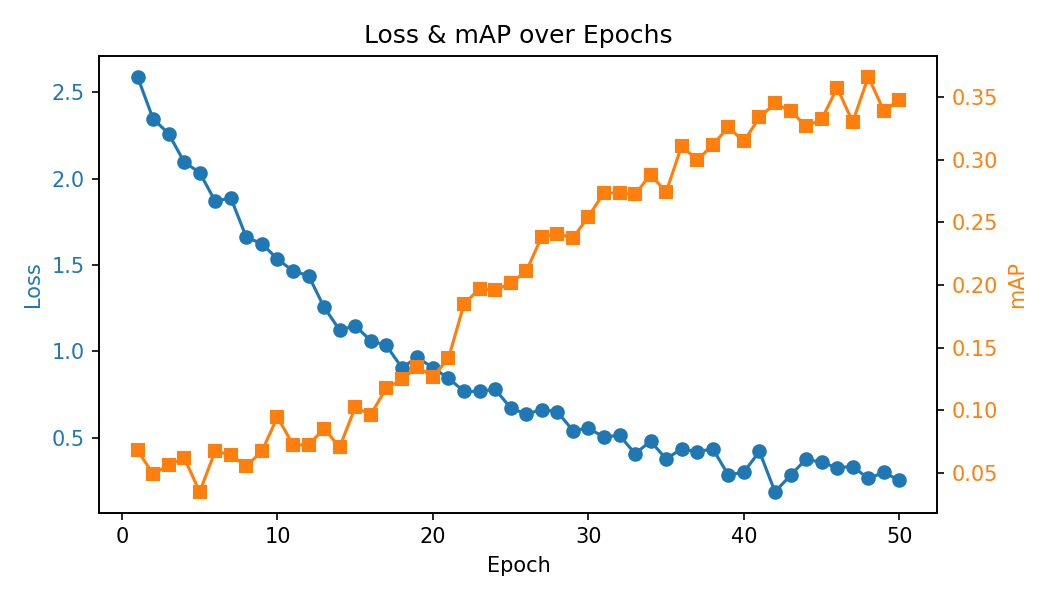
\includegraphics[width=0.65\linewidth]{../images/curves.png}
  \end{center}
\end{frame}

\begin{frame}{推理可视化示例}
  \begin{columns}
    \begin{column}{0.5\textwidth}
      \includegraphics[width=\linewidth]{../images/sample_dets/000003_det.jpg}\\[2mm]
      \includegraphics[width=\linewidth]{../images/sample_dets/000011_det.jpg}
    \end{column}
    \begin{column}{0.5\textwidth}
      \includegraphics[width=\linewidth]{../images/sample_dets/000014_det.jpg}\\[2mm]
      \includegraphics[width=\linewidth]{../images/sample_dets/000015_det.jpg}
    \end{column}
  \end{columns}
\end{frame}

% =========================
% Part III: 对齐与对比(约10分钟)
% =========================
\section{对齐与对比}

\begin{frame}{指标对齐(Jittor vs PyTorch)}
  \begin{table}[h]
    \centering
    \begin{tabular}{lccc}
      \toprule
      方法 & 输入尺寸 & mAP & AP50 \\
      \midrule
      PyTorch 复现(论文/官方) & 320 & \textit{(请填)} & \textit{(请填)} \\
      本工作 Jittor 复现 & 320 & \textbf{0.3476} & \textbf{0.563} \\
      \bottomrule
    \end{tabular}
  \end{table}
  \vspace{0.2cm}
  \textcolor{myred}{请提供你的 PyTorch 对齐实验日志/指标,我会补齐并加上误差来源分析。}
\end{frame}

\begin{frame}{可视化与误差分析}
  \begin{itemize}
    \item 典型成功案例:类别/定位与 PyTorch 一致
    \item 误差来源:数据预处理(比例/填充)、损失超参差异、NMS/阈值不同、数值精度(FP16 vs FP32)
    \item 进一步对齐:锁定随机种子、统一增广与调度器、统一 IoU/NMS 实现
  \end{itemize}
\end{frame}

\begin{frame}{结论与展望}
  \begin{itemize}
    \item 已实现 Jittor 端全链路可用,性能与预期一致
    \item 未来工作:
      \begin{itemize}
        \item 更系统的 PyTorch 对齐与消融
        \item TTA、量化/蒸馏、TensorRT 部署
        \item 多数据集泛化与小目标优化
      \end{itemize}
  \end{itemize}
\end{frame}

% 附录
\appendix
\section*{附录}
\begin{frame}{复现实验命令与仓库}
  \begin{itemize}
    \item 环境:conda activate nano,Jittor 1.3.10
    \item 全量验证:\texttt{bash DELIVERABLES/scripts/run\_full\_val.sh}
    \item Tiny overfit:\texttt{bash DELIVERABLES/scripts/run\_tiny20\_overfit.sh}
    \item 曲线/可视化:\texttt{bash DELIVERABLES/scripts/plot\_from\_log.sh},\texttt{bash DELIVERABLES/scripts/vis\_batch.sh}
    \item 交付目录:\texttt{DELIVERABLES/}
  \end{itemize}
\end{frame}

\end{document}

